\documentclass[11pt]{article}

\usepackage[utf8]{inputenc}
\usepackage[margin=2cm]{geometry} 
\usepackage{hyperref}
\usepackage{graphicx}
\usepackage{float}
\usepackage{caption}
\usepackage{longtable}
\usepackage{minted}
\usepackage{appendix}

\setlength{\parskip}{1em}
\setlength{\parindent}{0pt}

\title{Data Mining \& ML}
\author{ Group 4 }
\date{November 2020}

\begin{document}

\maketitle

\pagebreak

%TABLE OF CONTENTS
\tableofcontents
\thispagestyle{empty}
\pagebreak
\setcounter{page}{1}

\pagebreak

    

\section{File management, data pre-processing, transformation and selection} 
\subsection{File Management}

To easily reuse repetitive code across all Tasks we have developed modules (See Figure ~\ref{tab:moduleTable}) inside 
the Scripts directory which contains code that performs various tasks (See Appendix x.x). These functions help
in keeping our notebooks neat and tidy, for example, getting file paths for our data files or 
inserting data values into a dataframe to be used later on.
\par
To better understand the classified data we have implemented a confusion matrix as well as 
a function that displays all confusion matrices automatically for specified street signs, this 
provided quick analytics needed for Task 4 \& 5.

\subsection{Data pre-processing}

To preprocess the data we have implemented a function (found in helperfn.py) to handle imbalances 
within datasets thus it balances the class distribution of a chosen data so that it contains an 
equal number of images across all labels/classes.

\subsection{Transformations and selection}\label{sec:transSel}

\underline{Downsampling}
\par
We have used downsampling (downsampling.py) to get more information about exposing low level features.
By downsampling images using downsample.py we are able to reduce the image size by averaging 4 pixels into 1. This way we are able to find out what effect each area of the image has on the classification.
We have represented this in the form of a scatter graph, downsampling allows us to compare the average
greyscale value against their position(index of pixel) in the image.
\par 
We have also downsampled the image to a 12x12 image (See~\ref{12x12Scatter} )
By comparing the average greyscale to the row of the pixels, we can see where the
darkest pixels are located (Lower greyscale value is darker, higher is lighter).
\par
In the heatmaps we saw that the darkest pixels were the most definining which distinguishes 
each type of street sign.
\par
\underline{Binning}
\par
By implementing equal width binning we were able to convert the attributes from numerical to nominal type which enabled us to use Categorical Naive Bayes. 
Since the conditional probability distribution table is smaller, we learned that {\huge [Analysis/Conclusion Here]}

\pagebreak

\section{Naive Bayesian Networks}
To apply Naive Bayes classifier we have created a script called NaiveBayseCategorical.py 
/ NaiveBayseGaussian.py which takes care of building NB models using the sklearn Python Library
as well as splitting the data into training and testing which is required to appropriately find 
out how accurate a NB classifier is.
\par 
~\ref{train_2304}
\par
Observation: Having unbalanced class distribution negatively affects Naive Bayes across the board.


\pagebreak

\section{Complex Bayes nets}
\par
\emph{Describe \& analyse the problem. Show all experiments complete with graphs and tables. Discuss produced software quality \& discuss interesting properties of the data and algorithms}

\subsection{Building Bayse Networks}
Bayse networks represent probablistic directed acyclic graphs that define the relationshps between conditional dependencies and random variables. 
A naive Bayesian network can be represented in a Bayse network where the node representing the probability distribution of the class is the only parent of all other nodes and no other edges exist in the network. 
By adding additional edges (so long as the graph remains acyclic) we can represent causal relations between random variables.
\par
We decided to approach this task using both Weka and Python, with the intention of verifying our results against the other.
Attempting to build the network both ways gave us solid insights into the problems that would have to be solved to produce a Bayse Network.
We decided to use the pgmpy library to build our Bayse Networks in python, this immediately presented us with 2 computational complexity problems:
\begin{enumerate}
    \item Building all the conditional probability factors.
    \item Learning the optimal edges.
\end{enumerate}

*We handled the first problem by discretizing the greyscale values using equal width and frequency binning (see section~\ref{sec:transSel})*
When using Weka to compute Baysian networks we observed that Weka would perform extremely aggressive binning of the greyscale values often discretizing down to only 2 bins. This had a profound effect on the speed of learning the parameters and edges.

\subsection{Algorithms \& Data}


\subsection{Experimental Results}


\pagebreak

\section{Clustering}

\pagebreak
\appendix
\appendixpage
\addappheadtotoc
\begin{appendices}
\section{}
\subsection{Module Table}\label{tab:moduleTable}
The following are located in the Scripts folder
\begin{table}[ht]
    \centering
    \begin{tabular}{p{0.35\linewidth} | p{0.6\linewidth}} 
      \textbf{Module Name}  & \textbf{Description} \\ \hline
      helperfn.py & Provides functions to load and transform with all datasets required. \\ \hline
      downsample.py & Provides functions to downsample images  \\ \hline
      pixelFinder.py & Provides functions to find the most important pixels within a dataset of a chosen street sign. \\ \hline
      bayseNet.py & Provides functions used for getting a score for a model by testing all test data against labels. \\ \hline
      confusionMatrix.py & Provides functions for building and displaying confusion matrices as well as methods for calculating kappa values. \\ \hline
      plotScripts.py & Provides functions for plotting data into graphs \\ \hline
      wekaConversion.py & Provides functions to convert preprocessed data to be consumable by Weka
    \end{tabular}
\end{table}

\newpage
\subsection{Training data accuracy}\label{train_2304}
\begin{figure}[h!]
  \centering
  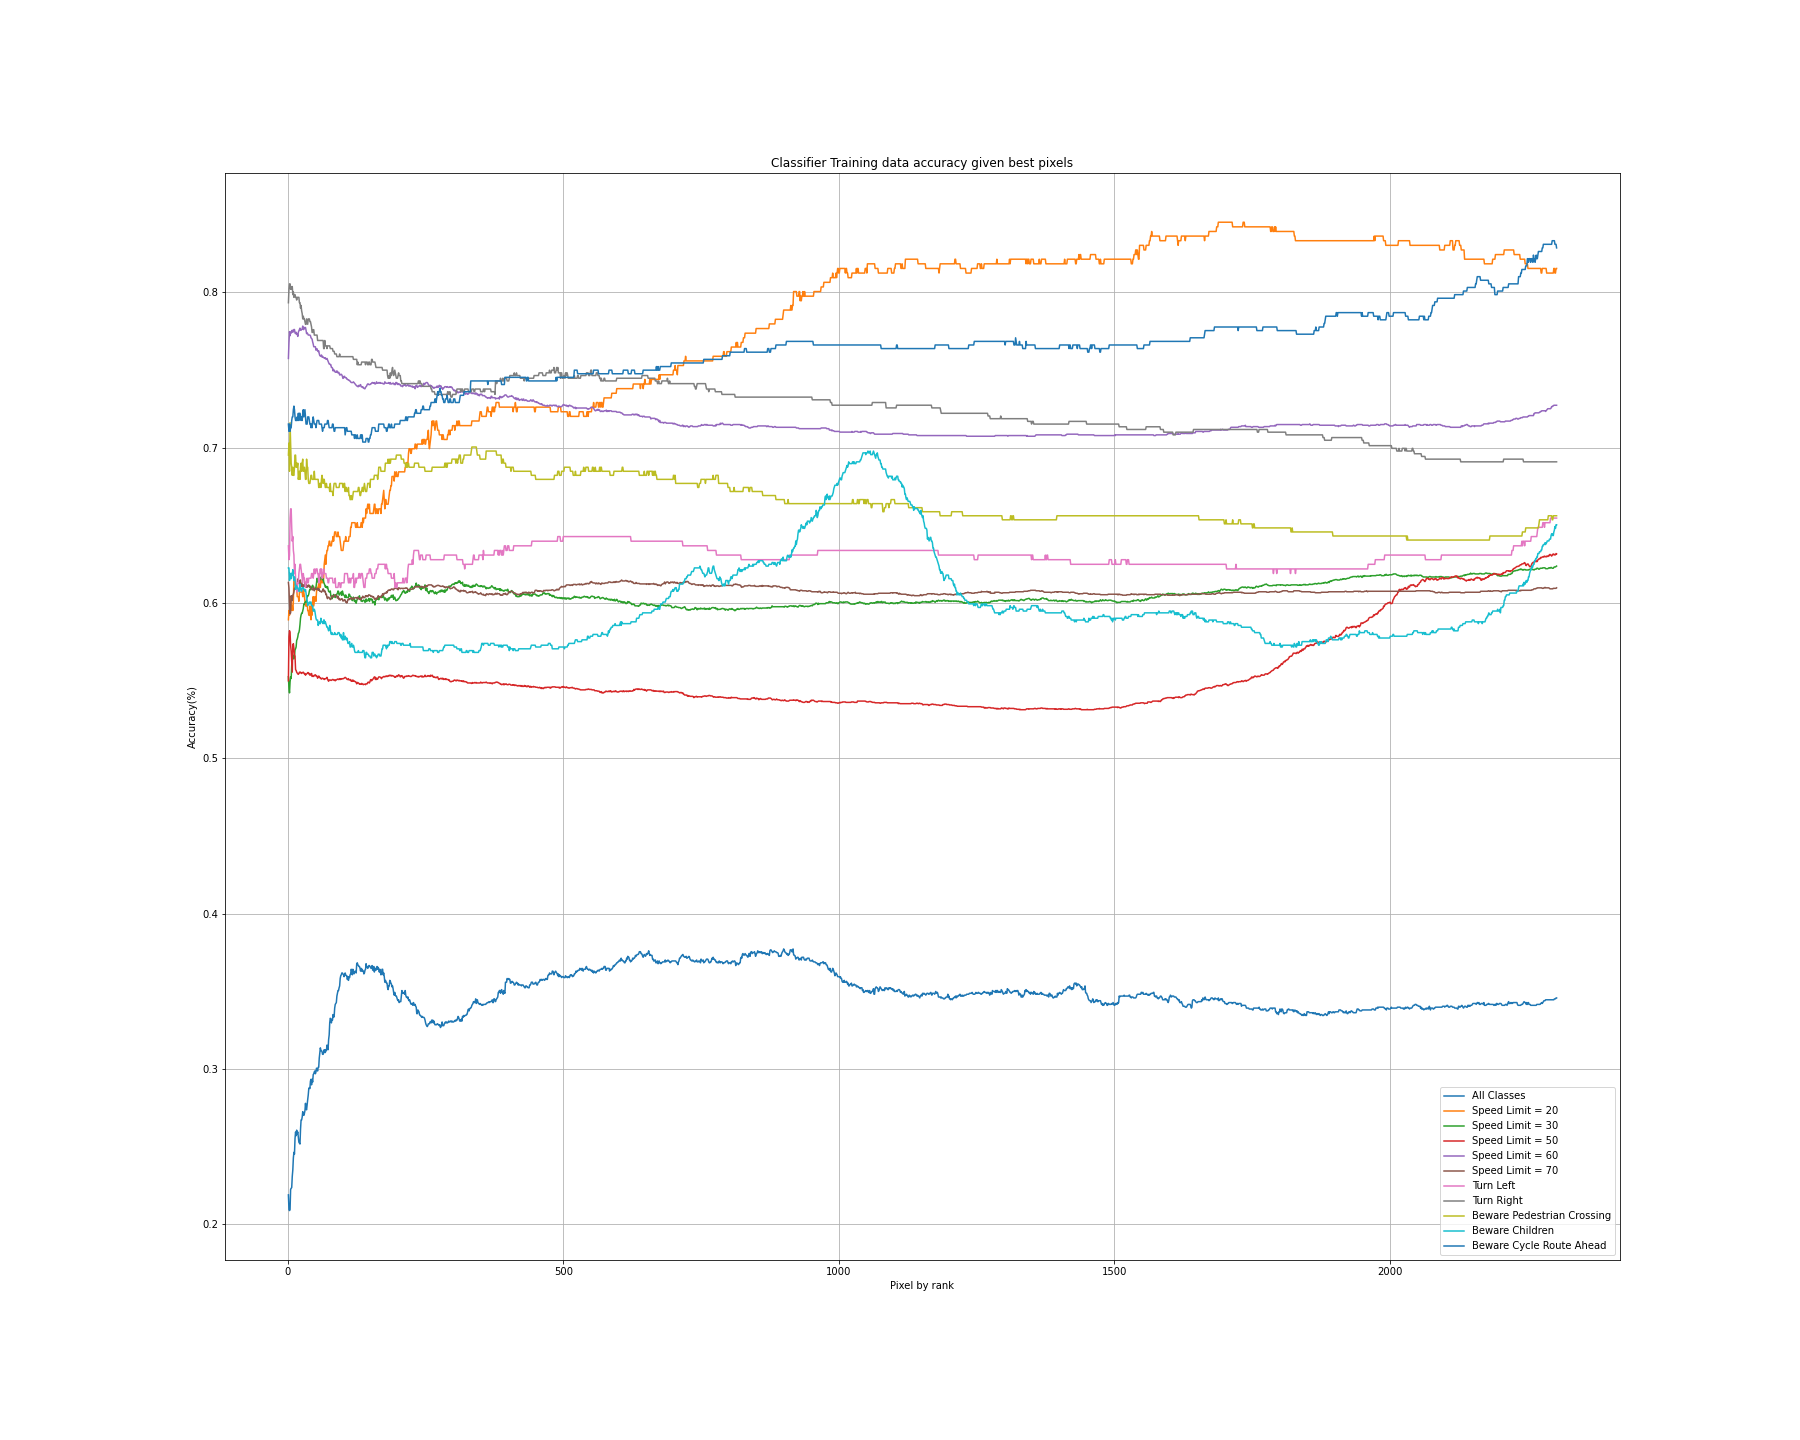
\includegraphics[scale=0.4]{Images/train_2304_pixels.png}
\end{figure}

\newpage
\subsection{12x12 Downsampled image}\label{12x12Scatter}
\begin{figure}[h!]
  \centering
  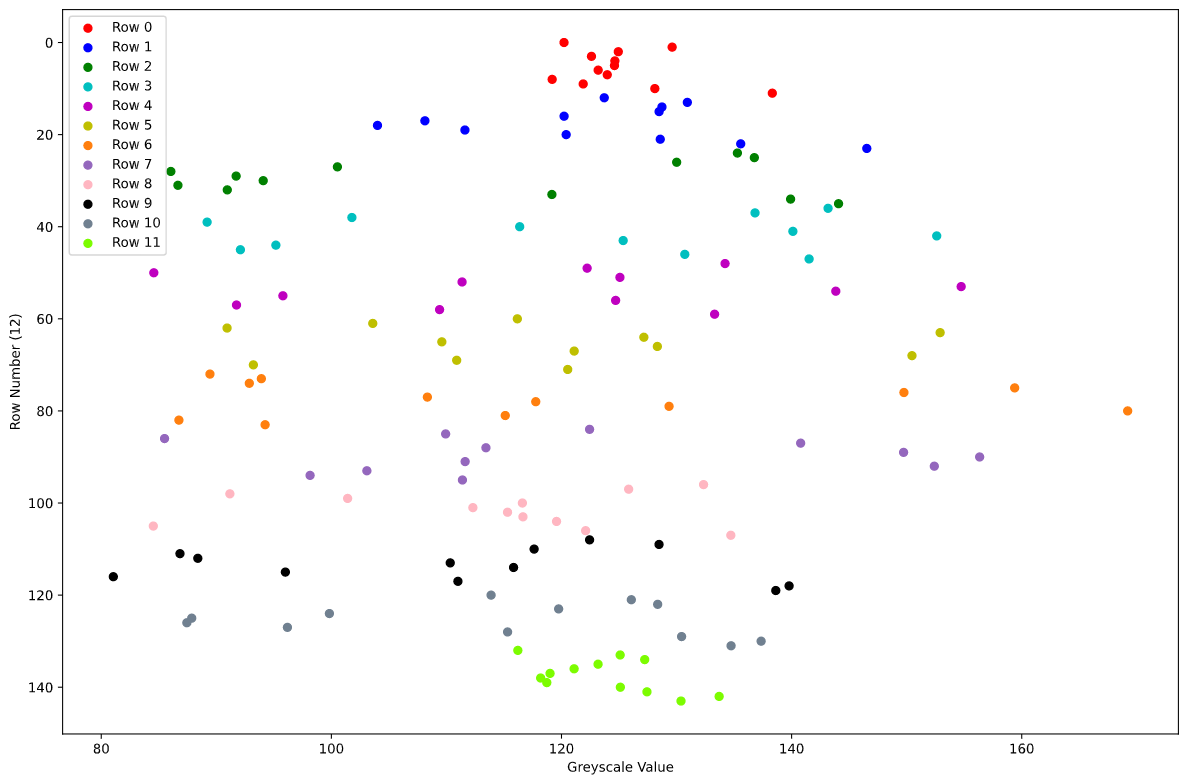
\includegraphics[scale=0.4]{Images/12x12 Scatter.png}
\end{figure}

\end{appendices}
\end{document}
